\documentclass[
	% -- opções da classe memoir --
	article,
	12pt,				% tamanho da fonte
	openright,			% capítulos começam em pág ímpar (insere página vazia caso preciso)
	twoside,			% para impressão em verso e anverso. Oposto a oneside
	a4paper,			% tamanho do papel. 
	% -- opções da classe abntex2 --
	%chapter=TITLE,		% títulos de capítulos convertidos em letras maiúsculas
	%section=TITLE,		% títulos de seções convertidos em letras maiúsculas
	%subsection=TITLE,	% títulos de subseções convertidos em letras maiúsculas
	%subsubsection=TITLE,% títulos de subsubseções convertidos em letras maiúsculas
	% -- opções do pacote babel --
	english,			% idioma adicional para hifenização
	spanish,			% idioma adicional para hifenização
	brazil,				% o último idioma é o principal do documento
	]{abntex2}

% ---
% PACOTES
% ---

% ---
% Pacotes fundamentais 
% ---
\usepackage{cmap}		% Mapear caracteres especiais no PDF
\usepackage{lmodern}		% Usa a fonte Latin Modern
\usepackage[T1]{fontenc}	% Selecao de codigos de fonte.
\usepackage[utf8]{inputenc}	% Codificacao do documento (conversão automática dos acentos)
\usepackage{indentfirst}	% Indenta o primeiro parágrafo de cada seção.
\usepackage{color}		% Controle das cores
\usepackage{graphicx}		% Inclusão de gráficos
\usepackage{booktabs}
\usepackage{colortbl}
\usepackage{setspace}
% ---

% ---
% Pacotes de citações
% ---
\usepackage[brazilian,hyperpageref]{backref}	 % Paginas com as citações na bibl
\usepackage[alf]{abntex2cite}	% Citações padrão ABNT

% --- 
% CONFIGURAÇÕES DE PACOTES
% --- 

% ---
% Configurações do pacote backref
% Usado sem a opção hyperpageref de backref
\renewcommand{\backrefpagesname}{Citado na(s) página(s):~}
% Texto padrão antes do número das páginas
\renewcommand{\backref}{}
% Define os textos da citação
\renewcommand*{\backrefalt}[4]{
	\ifcase #1 %

		% Nenhuma citação no texto.%
	\or
		%Citado na página #2.%
	\else
		%Citado #1 vezes nas páginas #2.%
	\fi}%
% ---



% Novo list of (listings) para QUADROS

\newcommand{\quadroname}{Quadro}
\newcommand{\listofquadrosname}{Lista de quadros}

\newfloat[chapter]{quadro}{loq}{\quadroname}
\newlistof{listofquadros}{loq}{\listofquadrosname}
\newlistentry{quadro}{loq}{0}

% configurações para atender às regras da ABNT
\counterwithout{quadro}{chapter}
\renewcommand{\cftquadroname}{\quadroname\space} 
\renewcommand*{\cftquadroaftersnum}{\hfill--\hfill}

% ---
% Informações de dados para CAPA e FOLHA DE ROSTO
% ---
\titulo{A técnica a serviço dos movimentos sociais: Combate aos impactos sócio-ambientais do agronegócio na amazônia maranhense}
\autor{Elias Lima de Souza}
\local{Campinas, Brasil}
\data{Abril de 2014}
\instituicao{%
Universidade Estadual de Campinas
  \par
Instituto de Geociências
  \par
  Programa de Pós-Graduação em Geografia}
\tipotrabalho{Projeto de Pesquisa}
\preambulo{Projeto de pesquisa para a elaboração de dissertação de Mestrado, no Programa de Pós-Graduação em Geografia do Instituto de Geociências da Universidade Estadual de Campinas, encaminhado para a Fundação de Amparo à Pesquisa do Estado de São Paulo}


\orientador[Orientador: Prof. Dr.]{Vicente Eudes Lemos Alves}




% ---
% Configurações de aparência do PDF final

% alterando o aspecto da cor azul
\definecolor{blue}{RGB}{41,5,195}

% informações do PDF
\makeatletter
\hypersetup{
    	%pagebackref=true,
	pdftitle={\@title}, 
	pdfauthor={Elias Lima de Souza},
    	pdfsubject={\imprimirpreambulo},
     pdfcreator={Elias Lima de Souza},
	pdfkeywords={abnt}{latex}{abntex}{abntex2}{projeto de pesquisa}, 
	colorlinks=false,       		% false: boxed links; true: colored links
    	linkcolor=blue,          	% color of internal links
    	citecolor=blue,        		% color of links to bibliography
    	filecolor=magenta,     		% color of file links
	urlcolor=blue,
	bookmarksdepth=4
}
\makeatother
% --- 

% --- 
% Espaçamentos entre linhas e parágrafos 
% --- 

% O tamanho do parágrafo é dado por:
\setlength{\parindent}{1.3cm}

% Controle do espaçamento entre um parágrafo e outro:
\setlength{\parskip}{0.2cm}  % tente também \onelineskip

% ---
% compila o indice
% ---
\makeindex
% ---

% ----
% Início do documento
% ----
\begin{document}

% Retira espaço extra obsoleto entre as frases.
\frenchspacing 

% ----------------------------------------------------------
% ELEMENTOS PRÉ-TEXTUAIS
% ----------------------------------------------------------
% \pretextual

% \imprimircapa
\imprimirfolhaderosto

\textual
\begin{resumoumacoluna}
Em tempos de desenvolvimento do agronegócio e conflitos de terra, o detentor da técnica exerce maior poder, legitimando seus interesses no território. Se a sociedade está, ainda que de forma seletiva, cada vez mais conectada à rede, acreditamos ser de fundamental a possibilidade de os movimentos sociais também terem meios de se apropriarem dessas técnicas, para que possam trabalhar com a informação com um potencial parecido com o dos agentes hegemônicos.

Devido à expansão do agronegócio no país, observa-se cada vez mais a ocorrência de  conflitos entre representantes da sociedade civil organizada, a exemplo de diversos movimentos sociais do campo e da cidade, e grandes empreendimentos agropecuários e agroindustriais além dos agentes do Estado, com  grandes projetos de infraestrutura executados pelo aparelho estatal.


Busca-se nesse projeto, a partir de orientações teóricas de Milton Santos e Manuel Castells sobre a técnica e a sociedade em rede, ajudar a reduzir a distância no acesso à técnica (e consequentemente ao poder) que existe atualmente entre os dois grupos de conflito (agentes do agronegócio e movimentos sociais). Para tanto, propõe-se a elaboração de uma ferramenta computacional que possibilite a organização e divulgação de informações nas redes sociais, visando facilitar a organização e amplitude de trabalho dos movimentos sociais da região de São Raimundo das Mangabeiras, na região sul do Maranhão.

 \vspace{\onelineskip}
 \noindent
 \textbf{Palavras-chaves}: Técnica. Movimentos sociais. Sociedade em rede. Poder e contrapoder. Agronegócio.
\end{resumoumacoluna}


\DoubleSpacing
\chapter{Apresentação da problemática}

O Brasil apresenta altos índices de desenvolvimento agrícola e com produção que vem crescendo constantemente. O sítio governamental \textbf{Portal Brasil}\footnote{http://www.brasil.gov.br/ - Acesso em 10. set. 2013} traz dados sobre a relevância do agronegócio para a economia do país e ressalta que o setor é responsável por mais de 22\% do Produto Interno Bruto brasileiro, assim como apresenta números expressivos em relação às vendas para o exterior, principalmente nas relações com a União Européia, China e Estados Unidos. Este Portal reforça que a política agrícola brasileira incentiva a expansão do setor, por meio da concessão de crédito e benefícios fiscais, além de programas como o "seguro rural".

O estado do Maranhão tem participação ativa e crescente no cenário do agronegócio brasileiro. As novas projeções para o agronegócio do Ministério da Agricultura Pecuária e Abastecimento, conforme \citeauthor{brministerioAgricultura2013} (\citeyear{brministerioAgricultura2013}), indicam a região conhecida como Mapitoba, que abrange parte dos estados do Maranhão, Piauí, Tocantins e Bahia, como uma das mais promissoras para o agronegócio do pais. Essa região se destaca atualmente principalmente pela produção de soja e arroz e tem uma dinâmica diferenciada de crescimento.

\begin{citacao}
"Seu crescimento tem sido extraordinário. A última pesquisa do IBGE (2011) sobre o PIB municipal mostra que esses 
municípios têm puxado o crescimento dos estados onde se localizam. Seu crescimento tem sido muito maior do que o crescimento do estado e da média brasileira. Esses quatro estados devem atingir uma produção de grãos de 18 milhões de toneladas nos próximos 10 anos numa área plantada de 7,3 milhões de hectares em 2022/2023, mas que poderá atingir 10,5 milhões de hectares em seu limite superior ao final da próxima década. [...] As áreas que vem sendo ocupadas nesses estados têm algumas características essenciais para a agricultura moderna. São planas e extensas, solos potencialmente produtivos, disponibilidade de água, e clima propício com dias longos e com elevada intensidade de sol. A limitação maior, no entanto são as precárias condições de logística, especialmente transporte terrestre, portuário, comunicação e, em algumas áreas ausência de serviços financeiros."
\cite[p. 64]{brministerioAgricultura2013}
\end{citacao}

As projeções ainda indicam que essa área deverá apresentar (\citeauthor{brministerioAgricultura2013} \citeyear{brministerioAgricultura2013}, p. 71) "aumento elevado da produção de grãos assim como sua área deve apresentar também aumento expressivo. As projeções indicam que essa região deverá produzir próximo de 18 milhões de toneladas de grãos em 2023 (aumento de 21,6\%) e uma área plantada de grãos entre 7 e 10 milhões de hectares ao final do período das projeções".

Dessa forma, o agronegócio é um setor da economia maranhense bastante estimulado, à medida que gera importantes recursos financeiros para o estado e é encarado pelo poder público como uma espécie de “salvação” para a região, historicamente marcada pela pobreza e grande concentração de renda. Porém, como lembram \citeauthoronline{rodrigues_alencar},

\begin{citacao}
a expansão do agronegócio da soja, a partir de grandes fazendas vem sendo responsável por vários problemas sócio-ambientais que se intensificam no Maranhão. A pressão que a abertura de grandes fazendas está fazendo nos recursos naturais do Cerrado, bem como a expropriação dos pequenos produtores e campesinos da região gera ainda mais problemas nas áreas de expansão da soja. O conflito entre fazendeiros e o campesinato, que tem feito sua história nesses lugares, muitas vezes há séculos, pode ser descrito como a face mais evidente da tensão, e que pode traduzir as várias formas do capitalismo entrar em conflito com as populações tradicionais \cite[p. 1]{rodrigues_alencar}
\end{citacao}

Com princípios de produtividade estabelecidos na “Revolução Verde”, o campo brasileiro vem se modernizando desde a década de 1970 e atingindo formas peculiares de produção. As novas técnicas de produção (maquinário, estradas, ferrovias, portos, pesquisas) artificializam o espaço, criando o meio técnico-científico-informacional de \citeauthoronline{santos1996} (\citeyear{santos1996}), onde os processos espaciais que produzem modificação da natureza são intensificados e criam formas atípicas e exógenas aos lugares:

\begin{citacao}
As modificações que acontecem no espaço agrário maranhense na atualidade são frutos da correlação de forças entre grandes projetos instituídos pelo planejamento estatal como modernizador do espaço maranhense e as populações tradicionais. No Cerrado essa hegemonia pelo território é dada pela tensão entre grandes proprietários e camponeses. A soja adentra esse quadro de modificações e arranjos espaciais como produto da 
modernidade, e em face da necessidade do modo de produção capitalista, em meio às transformações ocorridas nas últimas décadas, como parte de um processo de internacionalização dos espaços nacionais  \cite[p. 3]{rodrigues_alencar}
\end{citacao}

Como lembra \citeauthoronline{studte2008} (\citeyear{studte2008}), desde a década de 1980, a região sul do Maranhão foi transformando suas estruturas tradicionais de agricultura de subsistência em agricultura industrializada, que invariavelmente ocupa grandes extensões do territórios, substituindo ou pressionando áreas tradicionalmente destinadas a produção familiar camponesa. Esta transformação acontece em toda a área de fronteira agrícola do sul da Amazônia, de forma cada vez mais profunda dentro dos biomas amazônico e do cerrado.

\citeauthoronline{lima_locatel_silva} (\citeyear{lima_locatel_silva}, p.15) afirmam que as principais características que marcam o campo brasileiro na atualidade e, que são verificadas na região sul do Maranhão, correspondem à pauperização dos trabalhadores rurais e da estrutura fundiária concentrada e desigual, problemas estes que não foram resolvidos, mas "escamoteados a partir do desenvolvimento do capitalismo no campo".

Para Alfredo Wagner de \citeauthoronline{almeida}, a reconceituação de território atual tem sido marcada por novos critérios de classificação que reeditam a prevalência do quadro natural, “privilegiando biomas e ecossistemas como delimitadores de "regiões", flexibilizando as normas jurídicas que asseguram os direitos territoriais de povos e comunidades tradicionais e objetivando atender às demandas progressivas de um crescimento econômico baseado principalmente em commodities minerais e agrícolas” \cite{almeida}.

\citeauthoronline{rodrigues_alencar} também relatam que essa nova realidade de produção do espaço maranhense causa conflitos entre os camponeses e os agentes do agronegócio. Segundo os autores, 

\begin{citacao}
a luta do camponês contra o avanço do agronegócio se dá para ele como forma de se manter com seus meios de subsistência, para assim poder ser o protagonista da sua própria história, e não subordinar sua vida as demandas do grande capital, exógeno ao seu lugar e a sua cultura. [...] o conflito se manifesta de várias formas, primeiramente o conflito espacial pela produção, que se dá na forma velada, como anteriormente exposto, mas a forma violenta é a mais cruel, pois desaloja, desacredita e deixa órfãos. \cite[p. 10]{rodrigues_alencar}
\end{citacao}

\citeauthoronline{almeida} (\citeyear{almeida}), do mesmo modo, analisa as ações políticas que originam esse conflito entre produtor e camponês, afirmando que as pressões políticas que articulam a ação governamental visam uma "organização hierarquizada dos territórios". São ações rápidas com objetivos de curto prazo que exigem prontos "resultados estruturais (hidrelétricas, gasodutos, minerodutos, hidrovias, rodovias, portos, aeroportos, linhas de transmissão de energia), cujos efeitos referem-se a acidulados debates jurídicos e à intensificação de conflitos sociais" \cite{almeida}

Para o autor, o ritmo da ação governamental, aliada aos interesses privados que promovem a expansão das commodities, dá fundamento para pressões políticas em todo o país, que se manifestam através do mercado de terras e privilegiam algumas formas de ação:

\begin{alineas}
   \item a privatização das terras públicas sob o título de regularização fundiária;
   \item a redução de áreas protegidas ou unidades de conservação;
   \item a tentativas de incorporação de novas extensões territoriais aos circuitos mercantis - reforma do código florestal e redução das faixas de fronteira;
   \item a flexibilização dos direitos territoriais de povos e comunidades tradicionais.
\end{alineas}

Porém, o projeto de ocupação econômica dos cerrados maranhenses pode ser caracterizado

\begin{citacao}
pela negação das populações que aí se encontram, com a negação de sua cultura, identidade, e produção. Nos discursos dos programas de financiamento da agricultura da soja os espaços que estes se expandem são tidos como “Áreas de Cerrado Incorporadas ao Processo Produtivo", implicando uma clara concepção de "espaços vazios” [...] O Cerrado acaba sendo devastado pela paisagem homogênea e tecnificada que é criada,  também tem a diversidade social e cultural dos "Povos do Cerrado" comprometida. \cite[p. 13]{rodrigues_alencar}
\end{citacao}

Conforme \citeauthoronline{studte2008} (\citeyear{studte2008}), quase toda a área de vegetação natural restante na região encontra-se em áreas de ocupação dos pequenos produtores.  Tal autor ressalta  que é possível verificar que a modernização  da  agricultura na  região do sul do Maranhão, sobretudo, sob o comando  das grandes empresas foi concretizada  com foco no rendimento,  na produtividade, no lucro e na economia de mão-de-obra de trabalhadores rurais.  Ao passo que, os agricultores familiares não conseguem acompanhar esta velocidade de modernização.



Em tempos de desenvolvimento do agronegócio e conflitos de terra, o detentor da técnica exerce maior poder, legitimando seus interesses no território. Se a sociedade está, ainda que de forma seletiva, cada vez mais conectada à rede, acreditamos ser de fundamental importância a possibilidade de conexão dos movimentos sociais da região à rede, para que possam trabalhar com a informação com um potencial parecido com o dos agentes hegemônicos. Dessa forma, propomos um projeto com intenção fortalecer a inclusão dos movimentos sociais nas redes informacionais, permitindo o acesso à técnica pelos menos favorecidos.


\chapter{Objetivos}

\section{Gerais}

\begin{itemize}
 \item Compreender a dinâmica territorial da região e como a paisagem e a cultura local estão sendo alteradas conforme o agronegócio avança na região;
 \item Auxiliar na propagação no ciberespaço de informações geradas pelos movimentos sociais regionais acerca da ação do agronegócio;
 \item Permitir o acesso à técnica aos menos favorecidos visando diminuir a diferença de poder informacional entre os agentes do agronegócio e da sociedade civil organizada.
\end{itemize}

\section{Específicos}

\begin{itemize}
 \item Revisar a bibliografia sobre redes geográficas, a influência da técnica na composição do espaço, movimentos sociais em rede e impactos do agronegócio sobre um bioma;
 \item Mapear os pontos de avanço do agronegócio / áreas urbanas sobre a área de vegetação na região de estudo;
 \item Desenvolver uma ferramenta que tenha a função de um “portal” de informações sobre o impacto ambiental na região, com base em mapas colaborativos e dados estatísticos sobre o desmatamento na região que possa ser utilizada pela própria população, facilitando o acesso à técnica e à informação;
 \item Auxiliar no trabalho dos movimentos sociais, utilizando o portal de informações para disponibilizar no ciberespaço sobre os problemas causados pelo agronegócio na região de estudo, levando o movimento social para a rede com objetivo de integrar e expandir o movimento;
 \item Deixar um legado prático da pesquisa para a sociedade.
\end{itemize}


\section{Metodologia}

\citeauthoronline{isnard} (\citeyear{isnard}) afirma que o espaço geográfico é gerado pela sociedade, e sua produção e organização ao longo do tempo um campo de conflitos e embates. O espaço é, desse modo, “um amálgama de elementos que se movem, interagem e são solidários e contraditórios, por que criam espaços diferenciados, cada qual com sua função, com sua relação social” \cite{mondardo}

\citeauthoronline{santos1996} (\citeyear{santos1996}) definiu o espaço como um “conjunto indissociável de sistemas de objetos e sistemas de ações”, e a técnica, uma categoria analítica da associação entre esses sistemas, se mostra um elemento fundamental na explicação do espaço. Ainda assim, o autor frisa que “a técnica é um elemento importante de explicação da sociedade e dos lugares, mas, sozinha, a técnica não explica nada” \cite[p. 27]{santos1996}. Ela precisa ser estudada em conjunto com outros elementos do espaço, incluindo o tempo.

Ao analisar a afirmação de Pierre \citeauthoronline{george1974} (\citeyear{george1974}) "a influência da técnica sobre o espaço se exerce de duas maneiras e em duas escalas diferentes: a ocupação do solo pelas infra-estruturas das técnicas modernas [...] e as transformações generalizadas impostas pelo uso e execução dos novos métodos de produção e de existência" \cite[p. 13]{george1974}, \citeauthoronline{santos1996} (\citeyear{santos1996}, p.19) considera as conseqüências diretas do uso da técnica, como a própria instalação da infra-estrutura, e como conseqüências indiretas, as possibilidades que surgem com a implantação de um sistema técnico. 

Ainda segundo \citeauthoronline{santos1996} (\citeyear{santos1996}, p. 83), a técnica atua na produção do espaço modificando-o em termos de forma, função e paisagem, fatores determinantes de novas relações entre a sociedade e o espaço e entre a sociedade e si mesma. E como ressalta \citeauthoronline{marques} (2009, p. 21), “cada lugar revela uma técnica ou um conjunto de técnicas que o caracteriza particularmente e que contribui na formação de uma identidade própria [...] desta forma, a técnica constitui um dos elementos de explicação da sociedade e de cada um dos lugares”.
 
Hoje a informação é um elemento chave na composição da sociedade mundial e o meio técnico-científico-informacional é a “cara espacial da globalização” \cite{santos1996}, assim como a informação e os sistemas de comunicação adquirem importância fundamental na organização do espaço.

Ao estudar as teorias de Milton Santos, \citeauthoronline{maia} (\citeyear{maia}, p.9) sintetiza a história evolutiva do conceito "meio-técnico-científico-informacional", que “inicia-se na década de 1970; é caracterizado pela aplicação da ciência à técnica, por isto meio técnico científico; mas este meio, estas técnicas são impregnadas de informação e transmitem, acumulam informação, por isto meio-técnico-científico-informacional”. \citeauthoronline{santos1996} (\citeyear{santos1996}) define a relação entre os espaços, os agentes hegemônicos e o meio-técnico-científico-informacional:

\begin{citacao}
Os espaços assim requalificados atendem sobretudo aos interesses dos atores hegemônicos da economia, da cultura e da política e são incorporados plenamente às novas correntes mundiais. \cite[p. 191]{santos1996}
\end{citacao}

\citeauthoronline{maia} (\citeyear{maia}, p.5) ressalta ainda que a modificação acelerada do território, aliada à chegada e dispersão das técnicas de comunicação e informação, dá ao período atual uma forma diferenciada, que Milton Santos chama, em seu livro "A Natureza do Espaço", de instantaniedade dos momentos e dos lugares, universalidade e unicidade das técnicas.

Já \citeauthoronline{santos2001} (\citeyear{santos2001}) trabalha com a idéia que a técnica central e dominante nos dias atuais é a técnica da informação, e que o homem deixou de ser o centro do mundo, papel hoje é exercido pelo dinheiro, em uma geopolítica proposta por economistas e defendida pela mídia (detentora da técnica da informação). Dessa forma, as grandes empresas utilizam a mídia e, conseqüentemente a técnica, para realizar um tipo de dominação sobre o território, almejando se perpetuar como agente hegemônico.


Manuel \citeauthoronline{castells1999}, no livro A Sociedade Em Rede (\citeyear{castells1999}, p.50-51) considera a informação como um modo de desenvolvimento, moldado pela reestruturação do modo capitalista de produção, no final do século XX, que resulta no surgimento de uma nova estrutura social. Segundo o autor, a concepção teórica que fundamenta essa abordagem pressupõe que as sociedades são organizadas em processos estruturados por relações historicamente determinadas entre três elementos:

\begin{enumerate}

\item \textbf{Produção}, baseado na ação do homem sobre a natureza para apropriar-se dela e transforma-la seu beneficio;
\item \textbf{Experiência}, a ação dos humanos sobre si mesmos, determinada pela interação entre suas identidades biológicas e culturais em relação a seus ambientes sociais e naturais;
\item \textbf{Poder}, relação entre humanos que, com base na produção e na experiência, impõe a vontade de alguns sobre os outros, pelo emprego potencial ou real de violência física ou simbólica.

\end{enumerate}

Para o autor, a “comunicação simbólica entre os seres humanos e o relacionamento entre esses e a natureza,com base na produção (e seu complemento, o consumo), experiência e poder, cristalizam-se ao longo da história em territórios específicos, e assim geram culturas e identidades coletivas” \cite[p. 52-53]{castells1999}. Ele ainda ressalta como a difusão da tecnologia amplifica o poder de uma sociedade de forma infinita, a medida que os usuários apropriam-se da tecnologia e a redefinem: “pela primeira vez na história, a mente humana é uma força direta de produção, não apenas um elemento decisivo no sistema produtivo” \cite{castells1999}

A integração do território, motivada por interesses geopolíticos e pela necessidade de circulação de bens, pessoas e informação, deu-se através da implantação e extensão de redes geográficas, definidas por \citeauthoronline{correa} (1999) como um conjunto de localizações sobre a superfície terrestre articulado por vias e fluxos. Mais do que isso, a rede é um produto e também uma condição social, historicamente construída, dotada de intencionalidade e regulada politicamente \cite{santos1996}. \citeauthoronline{dias} (1995, p.150) frisa que a formação de redes no território é acompanhada de seletividade espacial, já que as redes não ligam todos os pontos. Elas exercem o papel de conexão de alguns pontos e de exclusão de outros, tornando mais estratégica a localização geográfica.

As redes constituem a morfologia social da sociedade atual e modificam de forma considerável a operação e os resultados dos processos produtivos e de experiência, poder e cultura. Elas são “estruturas abertas capazes de expandir de forma ilimitada, integrando novos nós desde que consigam comunicar-se dentro da rede” \cite[p. 566]{castells1999}. Essa última afirmação de Castells exemplifica o caráter excludente de uma rede, onde só é aceito o que se encaixa em seu padrão ou seus interesses. \citeauthoronline{santos1996} (1996) corrobora com essa análise, considerando as redes como agentes de inclusão e também de exclusão. \citeauthoronline{raffestin1993} (\citeyear{raffestin1993}, p.157) acredita que "toda rede é uma imagem do poder, ou mais exatamente, do poder do ou dos atores dominantes".

Para \citeauthoronline{castells1999} (1999, p. 70), as grandes áreas do mundo e consideráveis segmentos da população que estão desconectados do novo sistema tecnológico são regiões culturais e espacialmente descontínuas, enquanto grupos sociais e territórios dominantes estão constantemente conectados. Para o autor (1999, p. 476), sob a lógica do novo sistema o que importa não é a localização real dos centros de produção, mas a versatilidade de suas redes.

As sociedades são constituídas a partir das relações de poder entre seus membros, uma vez que os que detêm o poder constroem as instituições segundo seus valores e interesses. \citeauthoronline{castells2013} (2013, p.13) afirma que o “poder é exercido por meio da coerção e/ou pela construção de significado na mente das pessoas, mediante mecanismos de manipulação simbólica”.  Aqui, é importante citar \citeauthoronline{raffestin1993} (\citeyear{raffestin1993}, p. 212-213), para quem os nós não são meros pontos de conexão entre redes, mas também de poder.

Todavia, \citeauthoronline{castells2013} ressalta que as sociedades são contraditórias e conflitivas, de forma que onde há \textbf{poder}, há também o chamado \textbf{contrapoder}

\begin{citacao}
a capacidade de os atores sociais desafiarem o poder embutido nas instituições da sociedade com o objetivo de reivindicar a representação de seus próprios valores e interesses [...] A verdadeira configuração do Estado e de outras instituições que regulam a vida das pessoas depende dessa constante interação de poder e contrapoder \cite[p .13]{castells2013}.
\end{citacao}

Nos últimos anos, temos vivenciado um novo poder na geopolítica mundial. São os movimentos sociais organizados através das redes sociais na internet. Espaços onde há autonomia,

\begin{citacao}
muito além do controle de governos e empresas, que, ao longo da história, haviam monopolizado os canais de comunicação como alicerces de seu poder. Compartilhando dores e esperanças no livre espaço público da internet, conectando-se entre si e concebendo projetos a partir de múltiplas fontes do ser, indivíduos formaram redes, a despeito de suas opiniões pessoais ou filiações organizacionais \cite[p .10]{castells2013}
\end{citacao}

Nesse novo modelo de organização, as comunicações de massa são interativas e baseadas em redes horizontais de poder, mais difíceis de serem controladas por governos e/ou empresas. São exemplos dessa nova abordagem comunicativa o Coletivo Intervozes \footnote{http://intervozes.org.br/} e a Mídia Ninja \footnote{http://pt.wikipedia.org/wiki/M\%C3\%ADdia\_Ninja}, que ganharam destaque no país após a onda de manifestações populares de 2013 \footnote{http://pt.wikipedia.org/wiki/Manifesta\%C3\%A7\%C3\%B5es\_no\_Brasil\_em\_2013}.

Para \citeauthoronline{castells2013} (\citeyear{castells2013}, p.17-18), enquanto o poder é exercido programando e alterando redes, o contrapoder, uma tentativa de alterar as relações de poder predominantes, é realizado através da reprogramação das redes em torno de outros interesses e valor, que não os dos agentes hegemônicos. O contrapoder é exercido também pelos movimentos sociais, por meio de um processo de comunicação livre do controle dos que detêm o poder institucional, de forma que os movimentos possam ser construídos e agir na sociedade com menor influência do agente detentor de poder. 

Na sociedade em rede

\begin{citacao}
a autonomia de comunicação é basicamente construída nas redes da internet e nas plataformas de comunicação sem fio [...]  As redes sociais digitais oferecem a possibilidade de deliberar sobre e coordenar as ações de forma amplamente desimpedida. Entretanto, esse é apenas um componente do processo comunicativo pelo qual os movimentos sociais se relacionam com a sociedade em geral. Eles também precisam construir um espaço público, criando comunidades livres no espaço urbano. Uma vez que o espaço público institucional, o espaço constitucionalmente designado para a deliberação, está ocupado pelos interesses das elites dominantes e suas redes, os movimentos sociais precisam abrir um novo espaço público que não se limite à internet, mas se torne visível nos lugares da vida social \cite[p .18-19]{castells2013}.
\end{citacao}

A organização de movimentos sociais através das redes sociais permite ação e contatos mais ágeis e amplos do que a forma tradicional de organização (através de panfletos, boatos, reuniões). Porém, um dos grandes desafios é integrar e coordenar o trabalho tanto no ciberespaço quanto no espaço real, físico.

Boaventura de Sousa \citeauthoronline{boaventura2005} (\citeyear{boaventura2005}) analisa o uso das novas tecnologias de comunicação e de informação como 

\begin{citacao}
uma enorme oportunidade e um enorme risco. Uma não é possível sem o outro, mas é possível maximizar as oportunidades e minimizar os riscos. Para isso, é necessário criar e aplicar generalizadamente níveis de competência técnica e política nos cidadãos muito acima daqueles que a democracia liberal até agora foi capaz de gerar \cite[p.90]{boaventura2005}
\end{citacao}

O mesmo autor (\citeyear{boaventura2005}, p. 91) ainda justifica o uso das tecnologias pois elas "criam oportunidades insuspeitadas para desenvolver competência cidadã, competência para deliberar e tomar decisões políticas e não apenas para escolher os decisores políticos."

Como vimos, o acesso à técnica é desigual e seletivo. Assim, para auxiliar os movimentos sociais a se organizarem no espaço virtual, propomos a criação e utilização de um software que tenha a função de um "portal de informações" sobre a região, com notícias, estatísticas e que possibilite o mapeamento colaborativo das áreas afetadas pelo agronegócio, além de outras funcionalidades que surgirão a partir da necessidade dos usuários do sistema (no caso, integrantes dos movimentos sociais da região). A representação da sociedade local é fundamental pois "o saber local, que é nutrido pelo cotidiano, é a ponte para a produção de uma política – é resultado de sábios locais" (\citeauthor{santos1999}, \citeyear{santos1999}, p. 13). 

Os dados e informações disponíveis no software serão fornecidos de forma colaborativa pelos próprios agentes locais da comunidade, afim de alertar, denunciar e/ou divulgar as ações do agronegócio que afetam/destroem os bens naturais e o modo de vida da região. Através do uso desta ferramenta, será possível fortalecer a ação dos movimentos sociais na região através da auto-cartografia dos povos e comunidades tradicionais da amazônia, objetivando maior conhecimento sobre o processo histórico de ocupação dessa região. Com o uso da técnica e do poder informacional, acreditamos ser possível facilitar o exercício do contrapoder pelos movimentos sociais, agora em rede.


\chapter{Proposta de plano de trabalho}

\section{Descrição}

A elaboração da pesquisa aqui proposta pode ser subdividida em algumas seções e atividades a serem distribuídas ao longo de vinte e quatro meses de trabalho e contemplam levantamento de bibliografias e dados, trabalhos de campo, atividades de cunho prático e/ou técnico, além de análise de dados e redação de relatórios e artigos expondo a evolução do trabalho.

A seção de \textbf{levantamento bibliográfico e de dados} consiste em realizar um levantamento das produções bibliográficas, de teorias e métodos geográficos que:

\begin{itemize}
 \item Abordem a técnica e sua influência na configuração do território;
 \item Ressaltem as características da região estudada e as possibilidades e impedimentos dos movimentos sociais locais;
 \item Discutam evidências de impactos ambientais causados pelo agronegócio;
 \item Caracterizem a evolução do uso da técnica e como isso tem impactado a configuração espacial da região de estudo.
 \item Dissertem sobre as possibilidades de organização da sociedade em rede e o papel das redes sociais para a divulgação / organização de movimentos sociais;
\end{itemize}

Já a seção de \textbf{trabalhos práticos} consiste na elaboração de um software utilizando tecnologias livres que tenha a função de um "portal de informações" sobre a região, com notícias, estatísticas e que possibilite o mapeamento colaborativo das áreas afetadas pelo agronegócio, além de outras funcionalidades que surgirão a partir da necessidade de integrantes dos movimentos sociais de combate ao agronegócio da região. Os dados e informações disponíveis no software serão disponibilizados pelos próprios agentes locais da comunidade, afim de alertar, denunciar e/ou divulgar as ações do agronegócio que afetam/destroem os bens naturais e o modo de vida da região. Através do uso desta ferramenta, será possível fortalecer a ação dos movimentos sociais na região através da auto-cartografia dos povos e comunidades tradicionais da amazônia, objetivando maior conhecimento sobre o processo histórico de ocupação dessa região.

Uma das principais motivações para a construção desse software é a possibilidade de integrar às redes sociais as informações e os mapas construídos colaborativamente pela sociedade civil organizada, afim de auxiliar no trabalho de movimentos sociais que focam suas ações na evolução da situação na região em relação às ações do agronegócio. Com o uso da técnica e do poder informacional, acreditamos ser possível facilitar o exercício do contrapoder pelos movimentos sociais, agora em rede.

Este software será construído com base em metodologias ágeis\footnote{São metodologias de desenvolvimento de software baseadas em processos iterativos e incrementais de planejamento, execução, validação e reflexões sobre as decisões tomadas. Essas metodologias, como o SCRUM e a programação extrema, visam o contínuo incremento de valor ao produto, afim de maximizar a qualidade e a real utilidade do software.} de desenvolvimento, computação em nuvem\footnote{De forma simplória, a computação em nuvem é baseada na utilização de recursos de infra-estrutura e/ou serviços disponíveis na própria internet, eliminando a necessidade de criar uma estrutura física de servidores para publicar uma aplicação na internet.} e tecnologias livres\footnote{Tecnologias onde existe liberdade para utilizar, estudar, modificar e redistribuir a tecnologia original.}, sendo disponibilizado em ambiente de código-aberto\footnote{O código-fonte gerado para a construção do software estará disponível ao público na internet.}, para livre utilização pela comunidade.

Já para a seção de \textbf{trabalhos técnicos}, propõe-se a confecção de croquis e mapas sobre a evolução dos impactos sócio-ambientais na área de estudo, baseado nas informações obtidas através do software elaborado na seção de trabalhos práticos e nos trabalhos de campo realizados.

A \textbf{análise dos dados}, ocorrerá de forma constante, visando o direcionamento e a elaboração do trabalho da pesquisa. 

Para divulgação do resultado da pesquisa, pretende-se elaborar um ou mais artigos para submissão e publicação em periódicos especializados de geografia e/ou em computação, relatando algumas das considerações acerca da pesquisa, além da elaboração da dissertação de mestrado e apresentação dos resultados da pesquisa em eventos científicos com a temática da geografia, e do processo de construção do software em eventos de engenharia e desenvolvimento de software.

\section{Cronograma}

O cronograma prevê 24 meses de atividades, dispostas conforme o quadro abaixo:

\begin{figure}[htb]
\begin{center}
    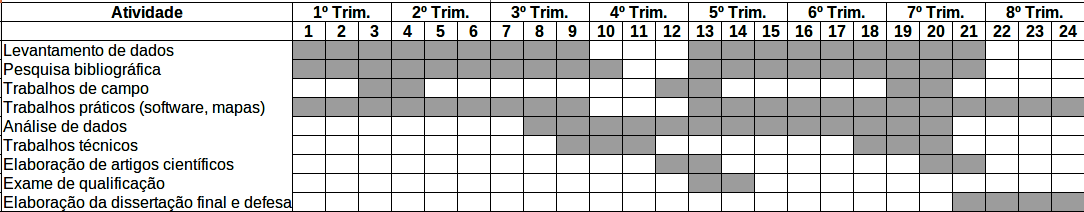
\includegraphics[scale=0.4]{crono.png}
\end{center}
\end{figure}

\begin{quadro}[!htbp]
\ABNTEXfontereduzida
\caption[Cronograma]{Cronograma de atividades}

\begin{tabular}{|l |c|c|c |c|c|c |c|c|c |c|c|c |c|c|c |c|c|c |c|c|c |c|c|c|}

\hline
\textbf{Atividade} &  \multicolumn{3}{|c|}{\textbf{1º Trim.}} & \multicolumn{3}{|c|}{\textbf{2º Trim.}} & \multicolumn{3}{|c|}{\textbf{3º Trim.}} & \multicolumn{3}{|c|}{\textbf{4º Trim.}} & \multicolumn{3}{|c|}{\textbf{5º Trim.}} & \multicolumn{3}{|c|}{\textbf{6º Trim.}} & \multicolumn{3}{|c|}{\textbf{7º Trim.}} & \multicolumn{3}{|c|}{\textbf{8º Trim.}}\\

\hline
{}  &  1 & 2  & 3  & 4  & 5  & 6  & 7  & 8  & 9  & 10  & 11  & 12  & 13  & 14  & 15  & 16  & 17  & 18  & 19  & 20  & 21 & 22 & 23 & 24 \\

\hline
Levantamento de dados  &  X & X & X & {}  & 6 & 8 & 8 & 8 & 8\\

\hline
Pesquisa bibliográfica  &  X & X & X & {}  & 6 & 8 & 8 & 8 & 8\\

\hline
Trabalhos técnicos (softwares, mapas)  &  X & X & X & {}  & 6 & 8 & 8 & 8 & 8\\

\hline
Análise de dados  &  X & X & X & {}  & 6 & 8 & 8 & 8 & 8\\

\hline
Elaboração de artigos científicos  &  X & X & X & {}  & 6 & 8 & 8 & 8 & 8\\

\hline
Exame de qualificação  &  X & X & X & {}  & 6 & 8 & 8 & 8 & 8\\

\hline
Elaboração e defesa da dissertação final  &  X & X & X & {}  & 6 & 8 & 8 & 8 & 8\\

\hline
\end{tabular}
\end{quadro}


\nocite{santos1996b, santos1998, mattelart2006, absaber, becker, goncalves, haesbaert}

\bibliography{bibliografia-geral}

% ---
% Finaliza a parte no bookmark do PDF, para que se inicie o bookmark na raiz
% ---
\bookmarksetup{startatroot}% 


\end{document}
